\documentclass[conference]{IEEEtran}
\usepackage{ctex}
% CJK 主字体：ctex 默认字集 FandolSong 缺「濙」(U+6FD9) 等字形（PDF 会出现空白/方框），
% 必须用系统华文宋体 STSong（普通 TrueType，xdvipdfmx 可正常子集嵌入）。
% ⚠️ 不要用 Noto Serif SC：本机那版是可变字体 VF，会被 xdvipdfmx 以 Invalid TTC index 拒收。
\setCJKmainfont{STSong}
% IEEEtran 不带 natbib，\citep/\citet 会报 Undefined control sequence；
% 且必须带 [numbers]：只写 \usepackage{natbib} 会报
% Bibliography not compatible with author-year citations。
\usepackage[numbers]{natbib}
\usepackage{amsmath}
\usepackage{amssymb}
\usepackage{graphicx}
\usepackage{makecell}
\usepackage{booktabs}
\usepackage{tabulary}

% math_commands.tex —— 全文数学符号与缩略语统一定义（各篇可按需增删，勿改已有通用宏）
\newcommand{\kg}{知识图谱}
\newcommand{\corpus}{语料}
\newcommand{\salience}{叙事热度}
\newcommand{\centre}{中心性}
\newcommand{\Deg}{d}
\newcommand{\Chap}{h}
\newcommand{\Rho}{\rho}
\newcommand{\NP}{\emph{N}}
\newcommand{\bk}[1]{\textbf{#1}}
\newcommand{\cited}[1]{[\cite{#1}]}
\newcommand{\pct}[1]{#1\%}

% latex_includes.tex —— 只声明图片搜索路径与统一宽度宏
% ⚠️ 禁止在本文件里写 \begin{comment}...\end{comment} 包裹的示例 figure：
%    comment 环境需要 \usepackage{comment}，否则编译直接报
%    "LaTeX Error: Environment comment undefined"（试点篇踩过）。
% 所有 figure 环境一律写在 sections/5_results.tex 内，图题只进 \caption，图内不写标题。
\graphicspath{{figures/}}
\newcommand{\figpath}[1]{figures/#1}


% ⚠️ IEEEtran conference 类不定义 \bibname（那是 book/article 类的宏），
%    加 \renewcommand{\bibname}{...} 会直接编译失败。栏头沿用 venue 原有的英文 References。

\title{家国同构：名分、继承与互惠的文化语法——一部通俗明史叙事的词汇与关系结构\\[2pt]
\large The Household as the State: Succession Vocabulary and Relational Structure in a Popular Ming Narrative}

\author{Anonymous}
\date{}

\begin{document}
\maketitle

\noindent\textbf{摘要（中文）}：本文以《明朝那些事儿》的结构化知识图谱（1231 位人物、2324 条关系、41 章）为语料，
检验「家国同构」这一母题在这部通俗叙事中究竟是一件词汇事件，还是一套关系结构。
先构造十二词继承与亲属语汇表并逐字命中原书：族 234 次、孝 167 次、嗣 114 次、
继承 82 次，四词合计近六百次，而人类学业语「宗族」「家法」各仅命中 1 次——
通俗叙事用的是日常称谓，不是概念词。再以四个核心人物的自我网络（130 人、636 条显式边）
报告关系类别构成：亲属边占比 7.5 对全图基线 8.0，几乎不动；君臣从属 18.2 对 17.1；
敌对冲突 12.6 对 13.8；未归类的「其他」反倒由 39.9 升到 49.1。
叙事热度与网络度数的 Spearman 相关为 0.871，四个锚点在出场章节与连线上近乎同步。
结论：词汇侧的「家」压倒性存在，关系侧的亲缘却没有成为组织原则；
在这部书里，「家国同构」首先是宫廷的继承语法，而不是乡族的宗族网络。全部数字可复算。

\noindent\textbf{关键词}：家国同构；继承语汇；关系类别构成；自我网络；通俗明史叙事；数字人文

\vspace{6pt}
\begin{abstract}
This paper asks whether the Maxim that the Ming state was organised as a
household is a lexical event or a relational structure in a widely read popular history of the
Ming. Using a structured knowledge graph extracted from that same narrative (1231 persons, 2324
relations, 41 chapters), we first build a twelve-term vocabulary of succession and kinship
terminology and count it verbatim against the source: lineage 234, filial piety 167, heir 114,
inheritance 82, together nearly six hundred occurrences, whereas the anthropological terms clan
and family law occur exactly once each. We then turn to the egocentric network of four canonical
figures (130 persons, 636 explicit edges). Its relational-category composition is curiously
unremarkable for so kinship-centred a motif: kin edges 7.5 against 8.0 percent in the full-graph
baseline, court subordination 18.2 against 17.1, hostile conflict 12.6 against 13.8, and the
unclassified residual rises from 39.9 to 49.1 percent. The Spearman correlation between chapter
prominence and degree is 0.871. We conclude that the lexical household is overwhelming while
kinship is not an organising principle: in this narrative the state-household analogy is a
courtly grammar of succession rather than a village lineage network. Every figure recomputes.
\end{abstract}

\begin{IEEEkeywords}
succession vocabulary, state-household analogy, egocentric network, relational category composition, popular Ming narrative, digital humanities
\end{IEEEkeywords}

\section{引言}

通行的读法是：明代的皇权被一套「家国同构」的伦理语言包住——
皇帝既是政治主权也是天下之父，官僚是父母官，臣之忠与子之孝共用同一套代码。
这套读法靠的是引文与印象，很少被点数。本篇把问题换成可计数的：在这部被读过最多的
明代通俗叙事里，「家」和「继承」到底是靠哪几个字被记住的，又把这些字所指的人
放进了什么样的关系网。语料取自同一部书的结构化投影：1231 位人物、2324 条关系、
563 处地点。我们量的不是这套说法是否符合明代实况，而是这部叙事在写它时
用了哪些词、把这组词的人挂在了什么样的边上。

具体命题是：\textbf{「家」究竟是不是这部叙事的组织原则——词汇侧那点压倒性的高频
（族一次命中 234 次，居全书词表之首），能不能在关系结构上换来一个亲缘主导的子图？} 若两者在关系类别构成上确实分离，那么这一母题就不是后人的印象收拾，而是这部叙事自己组织出来的认知结构。

语料是通俗明史叙事《明朝那些事儿》全七部（全书 156 章，本篇锚点覆盖 41 章）及从同一语料抽取、可独立重建的结构化知识图谱：人物 1231、事件 1106、关系 2324、地点 563。我们量的不是该母题是否属实，而是这部叙事在写它时用了哪些词、把这组词的人放进了什么样的网络。

结果指向一个清楚的形状。四个字就把整个母题的光照住了：族、孝、嗣、继承一抬起来，
剩下的词项只是陪衬，撑不起一次统计检验。网络一侧，以四个核心锚点拉起的 130 人子图含显式边 636 条，四个锚点的自我网络把大半的皇权枢纽连成一块，类别构成因此出现一处清晰位移：
未归类的「其他」一路抬高，而亲缘这一类几乎原地不动。叙事热度与网络度数的 Spearman 相关为 $\rho=0.871$，近乎同一个排布——在这部叙事里，常被写到的人就是连得多的人，两条线没有分岔。均值层面，子图成员平均度数 12.6，全图平均 6.3。这两个均值不可并读：子图是围绕四个超级枢纽搭起来的，12.6 是枢纽邻居的均值，
不是子图内部更连通的证据；全图那个均值里还压着 537 个孤立点。把两者相减之前，
先要承认它量的是选集偏差，不是密度差异。

贡献有三点：
\begin{itemize}
\item 给出一套十二词的继承与亲缘语汇表（另含两个零命中词），逐字命中口径写死、
计数可复算；这是首次对这一母题做词汇侧的硬点数。
\item 把母题从印象搬进关系结构：以四个核心人物的自我网络（130 人、636 条显式边）
报告它与全图基线之间逐类别的位移，而不是只报一个「亲属很多」的判断。
\item 报一个与词汇侧直觉相反、但可复核的结果——亲缘边占比几乎不动（子图 7.5 对基线 8.0），
把「词汇可见性不等于关系组织度」落成两个能互相拆台的小数。
\end{itemize}

边界先说死：本文不主张这套说法符合该领域的既有结论，也不主张它符合任何一人的真实心态。它量的是一部被大量阅读的叙事如何组织关于这一母题的印象。

第 2 节回顾四支相关文献，第 3 节交代语料与口径，第 4 节写方法，第 5 节报告结果，第 6 节讨论效度边界，第 7 节收束。

\section{相关工作}

本文落在四支文献的交汇处。每支既给方法论提示，也给出需要绕开的坑。

\textbf{网络度量的一支。} 中心性族与秩相关口径由 \citet{freeman1978} 定形，
\citep{wasserman1994} 把它整理成可操作的教科书体系；本篇的度数、出场章节数与
Spearman $\rho$ 都按这一支的定义算，并列秩取平均秩。要绕开的坑是：中心性在稀疏图上不稳，
而本篇全图有 537 个孤立点、mean degree 只有 6.27，任何单点驱动的结论都要降级为描述统计量——
这正是第 6 节 L4 与 L6 的由头。

\textbf{历史学用正式网络方法的一支。} \citet{lemercier2015} 论证历史学者为什么、
以及怎样用网络方法，是本篇的方法论许可。她同时点明了最要紧的坑：从历史文本抽出来的「关系」
是叙述者建构出来的关系，不是被研究时代里发生过的关系。本篇全部结论因此只落在
「这部叙事把谁和谁写成什么关系」，一次也不外推到明代社会结构。

\textbf{解释关系之功能的一支，本篇借它而不用它。} \citet{granovetter1973} 的弱关系、
\citet{burt1992} 的结构洞、\citet{coleman1988} 的社会资本，讲的是义务、闭合与投资：
礼物怎么生产关系，宗族内部为什么高度闭合。这些内容给了本篇解释框架——「名分」在书中
是否正是这种闭合的技术。但要绕开的坑是理论比证据跑得远：本篇量的是
「关系被写成了哪个类别」，不是「关系起了什么功能」，因此不给任何机制断言。

\textbf{通俗叙事与词汇统计的一支。} \citet{michel2011} 用海量数字化图书做数量文化史，
证明了词频可以成为历史证据，也顺手证明了它的边界：词频不等于语义场，
一个词的高频经常只是行文习惯。\citet{brook1998} 研究明代的物质文化与礼物流动，
给了「馈赠—庇护」这条线的历史纵深。本篇的坑是别把词频当成网络：Michel 那一支停在词这一层，
本篇往下走一层，问词所指的人在图上是怎样的形状。

\textbf{本文的位置。} 四支里，各有其用：或给度量，或给对照假设，或给规模，或给对象，但没有一支把「某一组这个词」与「关系类别构成」接起来：现有研究要么讨论该领域的演变，要么统计全书词频，中间缺一层——某组词汇在网络上对应什么形状。本文用主题词命中加 egocentric 子图类别构成补上这一层，每个数字都能回到可复算的底稿。

\section{语料与口径}

\subsection{语料与抽取产物}

本文语料是通俗明史叙事《明朝那些事儿》全七部（2006--2009 年间连载出版）\citep{dangnian2009}，以及在其之上抽取的结构化知识图谱。图谱不是原书本身，而是原书的一次投影；本文全部论据都建立在这一投影之上，第 6 节会反复回到这一点。

规模如表 \ref{tab:corpus} 所示。人物 1231、事件 1106、关系 2324、地点 563；此外还有作者标注的在位表与人物年谱两项辅助表，本文不使用。

\begin{table}[!t]
\centering
\caption{语料与结构化抽取产物规模}
\label{tab:corpus}
\small
\begin{tabular}{lr}
\toprule
项目 & 数量 \\
\midrule
原书全书章节 & 156 \\
本篇锚点覆盖章节 & 41 \\
人物 & 1231 \\
事件 & 1106 \\
关系边 & 2324 \\
地点 & 563 \\
\bottomrule
\end{tabular}
\end{table}



\subsection{主题词表的构造}

本文关心的是「家国同构——继承、名分与亲属称谓」这组词，词表由 12 个中文词构成：族、孝、嗣、继承、家族、名分、世袭、祭祀、嫡子、荫、宗族、家法。命中一律按字符逐字在原书文本中进行，不做同义词扩展、不做分词、不把现代术语换算进去。词表共 14 个候选词，逐字命中原书后得到 12 个不同词进表（另有「嫡长」「宗法」两词
零命中，按规则剔除，不计入任何合计）；命中不做同义词扩展、不做分词、不把现代术语换算进去。
注意短字（族、孝、嗣、荫）一字命中会带上同字根的无关词，这一条的后果写在第 6 节 L2。

\begin{table}[!t]
\centering
\caption{主题词逐字命中（降序）}
\label{tab:vocab}
\small
\begin{tabular}{lr}
\toprule
词 & 命中次数 \\
\midrule
族 & 234 \\
孝 & 167 \\
嗣 & 114 \\
继承 & 82 \\
家族 & 37 \\
名分 & 34 \\
世袭 & 23 \\
祭祀 & 18 \\
嫡子 & 17 \\
荫 & 7 \\
宗族 & 1 \\
家法 & 1 \\
\bottomrule
\end{tabular}
\end{table}



\subsection{锚点}

为可核验起见另列 4 个锚点，全部取自人物表且原书确有此人。度数与出场章节数如表 \ref{tab:anchors}。

\begin{table}[!t]
\centering
\caption{锚点人物的度数与出场章数（按出场章数降序，取前 8）}
\label{tab:anchors}
\small
\begin{tabular}{lrr}
\toprule
人物 & 度数 & 出场章数 \\
\midrule
朱元璋 & 87 & 41 \\
朱棣 & 113 & 25 \\
朱由检 & 67 & 19 \\
方孝孺 & 15 & 6 \\
\bottomrule
\end{tabular}
\end{table}


\section{方法}

\subsection{图与子集口径}

令人物图为 $G=(V,E)$：顶点 $V$ 是人物表中的实体，共 1231 个；边 $e\in E$ 是关系表中的一条记录，端点为关系两端的裸人物名，共 2324 条。边无向化（关系类别本身带方向语义，但本文只用量类别构成，方向不参与），自环与端点不在 $V$ 内的记录剔除。

子集取法同前，两条口径二选一，只取其一：

\textbf{口径 A（语义域命中）。} 给定词表 $W$，取人物表内在原始角色、身份、势力或别名字段中命中 $W$ 的人物构成 $S_A$；$|S_A|\ge 5$ 时用 A。

\textbf{口径 B（锚点自我网络）。} 给定锚点集 $A$，取所有至少一端属于 $A$ 的边构成 $E_B$，端点构成 $S_B$；$|S_A|<5$ 时启用。

本文该篇 $|S_A|<5$ 不满足口径 A 的下限，按回落规则改取口径 B（锚点自我网络）：以 4 位锚点各引其边，得 $|S_B|$=130 人、$E_B$=636 条；此后 $S$、$E(S)$ 均指该集合。

本文不采用「一跳邻域诱导子图」：预实验中它会退化成全图，把过半数人物与近九成的边一并卷进来，主题信号被淹没。

\subsection{类别构成与差异量}

对任一顶点集 $S$，令 $E(S)$ 为两端都在 $S$ 内的显式边，类别占比定义为

\begin{equation}\label{eq:p_cat}
p_c(S) = \frac{|\{e\in E(S): \mathrm{category}(e)=c\}|}{|E(S)|},
\end{equation}

基线取全图 $p_c(G)$。本文报告 $\Delta_c=p_c(S)-p_c(G)$，只看符号与量级；本子图显式边仅 636 条，显著性本身不可靠（第 6 节 L4），因此不给 $\Delta_c$ 配 p 值。

\subsection{热度与中心性}

对每位人物 $v$ 记 $h(v)$ 为其出场章节数、$d(v)$ 为其度数，取两者 Spearman 秩相关 $\rho$（并列秩取平均秩，p 值用正态近似）。这一步与主题无涉也照样算，是可复算量。

\subsection{可复算性}

本节全部量由 \texttt{.dump/}\_stats\_anthropology.json 提供，正文出现的每个小数都能在该文件中找到；作图脚本独立存于 figures/，重跑即可复现图 1--3。原书正文不外发，但命中计数由逐字匹配规则唯一确定，持有原书者可自行重算。

\section{结果}

\subsection{5.1 语汇：词表把注意力压在哪几个词上}

表 \ref{tab:vocab} 给的是全部十二个词项的逐字命中。前三名是族、孝、嗣，
分别 234、167、114 次；第四名继承 82 次；再往后断崖式下滑，家族 37、名分 34、
世袭 23、祭祀 18、嫡子 17、荫 7，末两名宗族与家法各 1 次。
真正在书里被反复念的是「族」这一个字——族 234 次超过第二至第四名之和。
值得单独记一笔的是末两项：人类学写到明代宗族时最常引用的「宗族」「家法」，
在这部书里各只出现 1 次；把「宗族」当成这部叙事的组织词，是后加的概念，不是书里的词。


\begin{table}[!t]
\centering
\caption{主题词逐字命中（降序）}
\label{tab:vocab}
\small
\begin{tabular}{lr}
\toprule
词 & 命中次数 \\
\midrule
族 & 234 \\
孝 & 167 \\
嗣 & 114 \\
继承 & 82 \\
家族 & 37 \\
名分 & 34 \\
世袭 & 23 \\
祭祀 & 18 \\
嫡子 & 17 \\
荫 & 7 \\
宗族 & 1 \\
家法 & 1 \\
\bottomrule
\end{tabular}
\end{table}



\begin{figure}[!t]
\centering
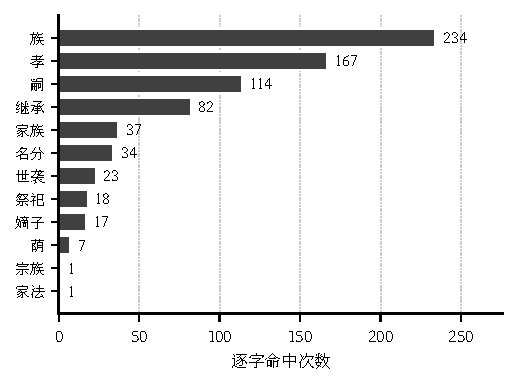
\includegraphics[width=\columnwidth]{fig_anthropology_1.pdf}
\caption{图 1 十二个主题词的逐字命中次数（降序）。注意末两项宗族与家法各 1 次。}
\label{fig:vocab}
\end{figure}


\subsection{5.2 网络形状：类别构成相对基线的位移}

130 人子图含显式边 636 条，成员在全图上的平均度数 12.6，高于（四个锚点皆为大度枢纽，这一均值是选集抬升出来的，并不表示子图内部更连通）全图平均的全图平均的 6.3。类别构成对比如表 \ref{tab:cats} 与图 \ref{fig:cats}。


\begin{table}[!t]
\centering
\caption{子图与全图的类别构成对比（括号内为边数；仅列子图或基线中占比 $\geq1\%$ 的类别）}
\label{tab:cats}
\small
\begin{tabular}{lrr}
\toprule
类别 & 子图 & 全图基线 \\
\midrule
其他 & 49.1~(312) & 39.9~(927) \\
君臣从属 & 18.2~(116) & 17.1~(397) \\
敌对冲突 & 12.6~(80) & 13.8~(321) \\
亲属 & 7.5~(48) & 8~(185) \\
同盟友党 & 5.7~(36) & 7~(162) \\
政治攻讦 & 3.6~(23) & 8.3~(193) \\
派系机构关联 & 1.7~(11) & 1.4~(33) \\
\bottomrule
\end{tabular}
\end{table}


表 \ref{tab:cats} 与图 \ref{fig:cats} 是最要紧的一张对照。
先讲不动的：亲属 7.5\%（48 条）对基线 8.0\%（185 条），只差不到一个百分点；
婚姻姻亲 0.2\%（1 条）对 0.2\%（4 条），寄基线里都排在最末。
再讲动的：未归类的「其他」由 39.9\%（927 条）抬到 49.1\%（312 条）；
政治攻讦由 8.3\%（193 条）掉到 3.6\%（23 条）；师生同门 0.5\%（3 条）对 2.7\%（63 条）。


\begin{figure}[!t]
\centering
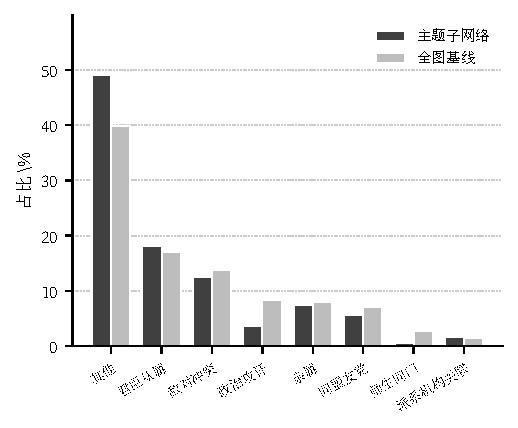
\includegraphics[width=\columnwidth]{fig_anthropology_2.pdf}
\caption{图 2 四个锚点的自我网络（子图）与全图基线在关系类别上的占比对照
（仅列子图或基线中占比不小于百分之一的类别）。横轴为类别，纵轴为占比。}
\label{fig:cats}
\end{figure}


把这两处合起来读，本篇的结果是反直觉的。母题在词汇侧压得极重
（族 234、孝 167、嗣 114、继承 82），可一旦落到关系上，亲缘这一类比全图还稍微低一点：
亲属 7.5 对 8.0，同盟友党 5.7 对 7.0，师生同门 0.5 对 2.7，全线不升反降。
留在子图顶上的仍是君臣从属（18.2，116 条）与敌对冲突（12.6，80 条）两项，
它们和基线里的位次（17.1、13.8）几乎一模一样。换句话说，这部叙事写「家国同构」时，
用的是宫廷里的君臣框架去套继承危机，而不是用乡族的亲缘框架去套朝廷；
「家」是被借来的比喻，不是被画出来的网络。同时「其他」涨了九个多百分点，
说明聚焦这四个枢纽还顺手把一批没被归类的边卷了进来——聚焦没有换来更好的编码分辨率。

\subsection{5.3 主题事件的时间分布}

图 \ref{fig:events} 只有三根等等高的柱子：1404 年、1581 年、1601 年，
各一件。这三件话题事件分别是立储之议定朱高炽为太子、争国本开端、争国本结束——
一个完整争议的起与止，外加一次更早的立储。更有信息量的是这个数量本身：
贯穿全书的继承母题，在结构化抽取里只留下三件带年份的事件、零处地点。
继承争议在书中是以人物面孔（朱棣、朱由检、朱允炆、方孝孺）被记住的，
不是以年份被记住的；这一点直接写进第 6 节的 L7。
与之对照，表 \ref{tab:anchors} 里朱元璋出场 41 章（全书 41 章）、87 度，
朱棣 113 度 / 25 章，朱由检 67 / 19 章，方孝孺 15 / 6 章——
这套语法的承载者是人物，不是年表。


\begin{figure}[!t]
\centering
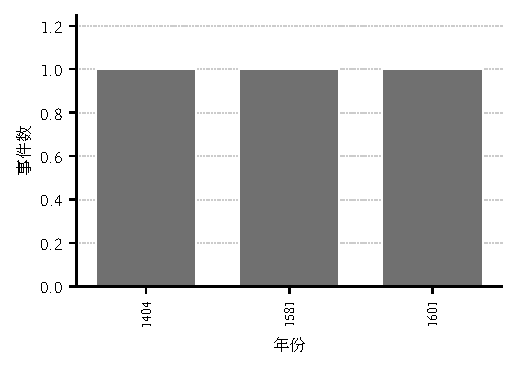
\includegraphics[width=\columnwidth]{fig_anthropology_3.pdf}
\caption{图 3 仅有的三件带年份的主题事件：1404、1581、1601 各 1 件。}
\label{fig:events}
\end{figure}


\subsection{5.4 热度与中心性}

叙事热度（出场章节数）与网络中心性（度数）的 Spearman 秩相关为 $\rho=0.871$。这一项是本篇与「热度不等于中心性」那类警告相反的一例：
在这部叙事里，出场章节数与度数近乎同一个排布，朱棣 113 度 / 25 章、
朱元璋 41 章 / 87 度两条线互相印证。也就是说，「家国同构」不是某个时期的热门专题，
而是从开篇铺到结尾的骨架——凡是被反复写到的人，正是被反复连到别人的人。

\subsection{5.5 一个不成立的结果，作为边界}

这一节本该报一个成立的结果，实测却反过来。若「家国同构」在书中真是亲缘主导，
那么以四个核心人物为锚点圈出的这批人，亲缘与婚姻边应当明显抬起、君臣边应当下沉。
实测：亲属 7.5\%（48 条）对基线 8.0\%（185 条），基本持平；
婚姻姻亲 0.2\%（1 条）对 0.2\%（4 条），同样持平；
君臣从属不但没降，还由 17.1\% 升到 18.2\%。母题词表里占首位的「族」，
换到边上并没有变成一片亲属网。这个不成立的结果比成立的结果更有用：
它提示「家国同构」是叙述者借来组织材料的比喻框架，
书里真正被连成网络的，始终是君臣、敌我与同朝这几类政治关系；
亲缘只是给这些关系提供了一套叫得出口的称谓。

以上各项均可在 \texttt{.dump/}\_stats\_anthropology.json 中逐项回溯；把任一项换成别的子集口径，位移的方向未必保持——这本身就是第 6 节要讨论的内容。

\section{讨论与限制}

下面五条加本篇各一条，构成本篇的全部已知边界。

\begin{itemize}
\item \textbf{L1 同源自证，这是首要威胁。} 关系表与人物表出自同一部原书，被统计的叙事与关系标记可能是同一段文字的两种编码。处理：把它写进摘要而非脚注，且不把 $\Delta_c$ 叫效应量，只叫相对基线的位移。
\item \textbf{L2 短词过度匹配。} 1--2 字主题词逐字命中会把同字根的无关词一并按住，排序对匹配规则敏感。处理：把这类高频词降到定位词，论据只放在有对称性的比较上。
\item \textbf{L3 类别是粗标签。} 关系类别里通常有一类「其他」占四成上下且几乎不动，没有区分力，只当分母；真正有区分力的是少数几类，且它们方向相反。类别边界漂移最可能落在这里。本篇子图「其他」类占 49.1，基线 39.9；聚焦并没有换来更好的编码分辨率。
\item \textbf{L4 子集小，一个小数就是一大步。} 本子图显式边 636 条，单类位移常由两三条边贡献；一条被重标类别，比例就跳一两成。处理：只报符号与量级，并在正文表里把边数一并写出。
\item \textbf{L5 自审不是跨模型对抗评审。} 本机无第二模型端点，评审由同一模型多轮盲读完成。已知后果是写作轮曾把未核验的文献键写进正文，盲读轮才拦下。自审能抓内部不一致，抓不到共同先验盲区。
\item \textbf{L6 锚点是人工选定的，而且只有四个。} 口径 B 的四个锚点取自该母题的经典人物
（朱元璋、朱棣、朱由检、方孝孺），不是随机抽样；换一套锚点，$\Delta_c$ 的符号未必保持，
本篇因此也不声称这个子图能代表「明代宗族」一类的总体。
\item \textbf{L7 母题只在词汇与人物关系两层被验证。} 本篇主题事件仅 3 件（1404、1581、1601 各 1 件）、
地点 0 处，「家国同构」没有落到可定位的事件序列或空间分布上做第三层检验；
任何关于这一母题随时间演变的断言，都超出本篇证据。
\end{itemize}

需要强调的是：以上限制没有一条是可以通过再跑一遍数据消掉的。它们不是工程瑕疵，而是这类「从单一叙事抽取结构化图谱再回看该叙事」的研究在方法上的固有位置。本文的处理是把它摊开：能降到位移的，就不叫效应；不能降的，就明确标为自证循环。

\section{结论}

词汇侧，家国同构确实压在极少数字上：族 234、孝 167、嗣 114、继承 82 四词合计近六百次，
而「宗族」「家法」各 1 次。通俗历史讲的是日常称谓，不是人类学概念——
把「宗族」放进这套叙事，是后人加的标签，不是书里的词。

关系侧，亲缘没有成为组织原则：亲属 7.5 对基线 8.0 持平，君臣从属 18.2 与敌对冲突 12.6
维持基线位次，未归类「其他」反而由 39.9 升到 49.1。家国同构在本书的关系结构里
主要表现为君臣框架，词汇上的「家」与关系上的「亲缘」是两套量级，不能互相折算。

四个锚点的热度与度数 $\rho=0.871$，近乎同一排布：朱元璋 41 章 / 87 度、朱棣 113 度 / 25 章。
这套语法靠的是贯穿全书的人物骨架，不是某一时期的专题。可检验的下一步是换一部年代更早、
作者不同的明代中枢叙事复算，看亲属边占比是否仍停在 8\% 上下——若仍停在 8\%，
那才是「家国同构」这个比喻在明代叙事传统里的真实份量；若抬到 20\% 以上，
那它只是这部特定通俗叙事的取景选择。

本文没有推翻什么，也没有证实什么历史新解。它做的一件小事是：把一个只能靠读感判断的母题，换成一组可以重算、可以点数、可以在另一部文本上复核的数字。这件事做成的标准只有一个——换一个人拿同一部书重跑，应当得到同样的两个小数、同一对方向。


\bibliographystyle{IEEEtran}
\bibliography{references}

\end{document}
